% Options for packages loaded elsewhere
\PassOptionsToPackage{unicode}{hyperref}
\PassOptionsToPackage{hyphens}{url}
%
\documentclass[
]{article}
\usepackage{amsmath,amssymb}
\usepackage{lmodern}
\usepackage{iftex}
\ifPDFTeX
  \usepackage[T1]{fontenc}
  \usepackage[utf8]{inputenc}
  \usepackage{textcomp} % provide euro and other symbols
\else % if luatex or xetex
  \usepackage{unicode-math}
  \defaultfontfeatures{Scale=MatchLowercase}
  \defaultfontfeatures[\rmfamily]{Ligatures=TeX,Scale=1}
\fi
% Use upquote if available, for straight quotes in verbatim environments
\IfFileExists{upquote.sty}{\usepackage{upquote}}{}
\IfFileExists{microtype.sty}{% use microtype if available
  \usepackage[]{microtype}
  \UseMicrotypeSet[protrusion]{basicmath} % disable protrusion for tt fonts
}{}
\makeatletter
\@ifundefined{KOMAClassName}{% if non-KOMA class
  \IfFileExists{parskip.sty}{%
    \usepackage{parskip}
  }{% else
    \setlength{\parindent}{0pt}
    \setlength{\parskip}{6pt plus 2pt minus 1pt}}
}{% if KOMA class
  \KOMAoptions{parskip=half}}
\makeatother
\usepackage{xcolor}
\usepackage[margin=1in]{geometry}
\usepackage{color}
\usepackage{fancyvrb}
\newcommand{\VerbBar}{|}
\newcommand{\VERB}{\Verb[commandchars=\\\{\}]}
\DefineVerbatimEnvironment{Highlighting}{Verbatim}{commandchars=\\\{\}}
% Add ',fontsize=\small' for more characters per line
\usepackage{framed}
\definecolor{shadecolor}{RGB}{248,248,248}
\newenvironment{Shaded}{\begin{snugshade}}{\end{snugshade}}
\newcommand{\AlertTok}[1]{\textcolor[rgb]{0.94,0.16,0.16}{#1}}
\newcommand{\AnnotationTok}[1]{\textcolor[rgb]{0.56,0.35,0.01}{\textbf{\textit{#1}}}}
\newcommand{\AttributeTok}[1]{\textcolor[rgb]{0.77,0.63,0.00}{#1}}
\newcommand{\BaseNTok}[1]{\textcolor[rgb]{0.00,0.00,0.81}{#1}}
\newcommand{\BuiltInTok}[1]{#1}
\newcommand{\CharTok}[1]{\textcolor[rgb]{0.31,0.60,0.02}{#1}}
\newcommand{\CommentTok}[1]{\textcolor[rgb]{0.56,0.35,0.01}{\textit{#1}}}
\newcommand{\CommentVarTok}[1]{\textcolor[rgb]{0.56,0.35,0.01}{\textbf{\textit{#1}}}}
\newcommand{\ConstantTok}[1]{\textcolor[rgb]{0.00,0.00,0.00}{#1}}
\newcommand{\ControlFlowTok}[1]{\textcolor[rgb]{0.13,0.29,0.53}{\textbf{#1}}}
\newcommand{\DataTypeTok}[1]{\textcolor[rgb]{0.13,0.29,0.53}{#1}}
\newcommand{\DecValTok}[1]{\textcolor[rgb]{0.00,0.00,0.81}{#1}}
\newcommand{\DocumentationTok}[1]{\textcolor[rgb]{0.56,0.35,0.01}{\textbf{\textit{#1}}}}
\newcommand{\ErrorTok}[1]{\textcolor[rgb]{0.64,0.00,0.00}{\textbf{#1}}}
\newcommand{\ExtensionTok}[1]{#1}
\newcommand{\FloatTok}[1]{\textcolor[rgb]{0.00,0.00,0.81}{#1}}
\newcommand{\FunctionTok}[1]{\textcolor[rgb]{0.00,0.00,0.00}{#1}}
\newcommand{\ImportTok}[1]{#1}
\newcommand{\InformationTok}[1]{\textcolor[rgb]{0.56,0.35,0.01}{\textbf{\textit{#1}}}}
\newcommand{\KeywordTok}[1]{\textcolor[rgb]{0.13,0.29,0.53}{\textbf{#1}}}
\newcommand{\NormalTok}[1]{#1}
\newcommand{\OperatorTok}[1]{\textcolor[rgb]{0.81,0.36,0.00}{\textbf{#1}}}
\newcommand{\OtherTok}[1]{\textcolor[rgb]{0.56,0.35,0.01}{#1}}
\newcommand{\PreprocessorTok}[1]{\textcolor[rgb]{0.56,0.35,0.01}{\textit{#1}}}
\newcommand{\RegionMarkerTok}[1]{#1}
\newcommand{\SpecialCharTok}[1]{\textcolor[rgb]{0.00,0.00,0.00}{#1}}
\newcommand{\SpecialStringTok}[1]{\textcolor[rgb]{0.31,0.60,0.02}{#1}}
\newcommand{\StringTok}[1]{\textcolor[rgb]{0.31,0.60,0.02}{#1}}
\newcommand{\VariableTok}[1]{\textcolor[rgb]{0.00,0.00,0.00}{#1}}
\newcommand{\VerbatimStringTok}[1]{\textcolor[rgb]{0.31,0.60,0.02}{#1}}
\newcommand{\WarningTok}[1]{\textcolor[rgb]{0.56,0.35,0.01}{\textbf{\textit{#1}}}}
\usepackage{graphicx}
\makeatletter
\def\maxwidth{\ifdim\Gin@nat@width>\linewidth\linewidth\else\Gin@nat@width\fi}
\def\maxheight{\ifdim\Gin@nat@height>\textheight\textheight\else\Gin@nat@height\fi}
\makeatother
% Scale images if necessary, so that they will not overflow the page
% margins by default, and it is still possible to overwrite the defaults
% using explicit options in \includegraphics[width, height, ...]{}
\setkeys{Gin}{width=\maxwidth,height=\maxheight,keepaspectratio}
% Set default figure placement to htbp
\makeatletter
\def\fps@figure{htbp}
\makeatother
\setlength{\emergencystretch}{3em} % prevent overfull lines
\providecommand{\tightlist}{%
  \setlength{\itemsep}{0pt}\setlength{\parskip}{0pt}}
\setcounter{secnumdepth}{-\maxdimen} % remove section numbering
\usepackage{booktabs}
\usepackage{longtable}
\usepackage{array}
\usepackage{multirow}
\usepackage{wrapfig}
\usepackage{float}
\usepackage{colortbl}
\usepackage{pdflscape}
\usepackage{tabu}
\usepackage{threeparttable}
\usepackage{threeparttablex}
\usepackage[normalem]{ulem}
\usepackage{makecell}
\usepackage{xcolor}
\ifLuaTeX
  \usepackage{selnolig}  % disable illegal ligatures
\fi
\IfFileExists{bookmark.sty}{\usepackage{bookmark}}{\usepackage{hyperref}}
\IfFileExists{xurl.sty}{\usepackage{xurl}}{} % add URL line breaks if available
\urlstyle{same} % disable monospaced font for URLs
\hypersetup{
  pdftitle={The Relationship between Urban Green Space and Socioeconomic Factors in the City of Vancouver: A Case of Environmental Injustice},
  pdfsubject={ENVSOCTY 4GA3: Applied Spatial Statistics},
  hidelinks,
  pdfcreator={LaTeX via pandoc}}

\title{The Relationship between Urban Green Space and Socioeconomic
Factors in the City of Vancouver: A Case of Environmental Injustice}
\author{true \and true \and true \and true}
\date{18 April, 2023}

\begin{document}
\maketitle

\hypertarget{r-markdown}{%
\subsection{R Markdown}\label{r-markdown}}

This is an R Markdown document. Markdown is a simple formatting syntax
for authoring HTML, PDF, and MS Word documents. For more details on
using R Markdown see \url{http://rmarkdown.rstudio.com}.

When you click the \textbf{Knit} button a document will be generated
that includes both content as well as the output of any embedded R code
chunks within the document. You can embed an R code chunk like this:

\begin{Shaded}
\begin{Highlighting}[]
\CommentTok{\# Clearing data}
\FunctionTok{rm}\NormalTok{(}\AttributeTok{list =} \FunctionTok{ls}\NormalTok{())}
\end{Highlighting}
\end{Shaded}

Note that the \texttt{echo\ =\ FALSE} parameter was added to the code
chunk to prevent printing of the R code that generated the plot.

\begin{Shaded}
\begin{Highlighting}[]
\CommentTok{\# loading packages}
\FunctionTok{library}\NormalTok{(cancensus) }\CommentTok{\#this package allows us to download census data from Stats Canada}
\end{Highlighting}
\end{Shaded}

\begin{verbatim}
## Census data is currently stored temporarily.
## 
##  In order to speed up performance, reduce API quota usage, and reduce unnecessary network calls, please set up a persistent cache directory by setting the environment variable CM_CACHE_PATH= '<path to cancensus cache directory>' or  setting options(cancensus.cache_path = '<path to cancensus cache directory>')
## 
##  You may add this environment varianble to your .Renviron or add this option, together with your API key, to your .Rprofile.
\end{verbatim}

\begin{Shaded}
\begin{Highlighting}[]
\FunctionTok{library}\NormalTok{(ggplot2) }
\FunctionTok{library}\NormalTok{(tidyverse) }\CommentTok{\#collection of packages for data visualization and manipulation (includes dplyr and ggplot2)}
\end{Highlighting}
\end{Shaded}

\begin{verbatim}
## -- Attaching core tidyverse packages ------------------------ tidyverse 2.0.0 --
## v dplyr     1.1.0     v readr     2.1.4
## v forcats   1.0.0     v stringr   1.5.0
## v lubridate 1.9.2     v tibble    3.2.0
## v purrr     1.0.1     v tidyr     1.3.0
\end{verbatim}

\begin{verbatim}
## -- Conflicts ------------------------------------------ tidyverse_conflicts() --
## x dplyr::filter() masks stats::filter()
## x dplyr::lag()    masks stats::lag()
## i Use the ]8;;http://conflicted.r-lib.org/conflicted package]8;; to force all conflicts to become errors
\end{verbatim}

\begin{Shaded}
\begin{Highlighting}[]
\FunctionTok{library}\NormalTok{(tidycensus)}
\FunctionTok{library}\NormalTok{(tigris)}
\end{Highlighting}
\end{Shaded}

\begin{verbatim}
## To enable caching of data, set `options(tigris_use_cache = TRUE)`
## in your R script or .Rprofile.
\end{verbatim}

\begin{Shaded}
\begin{Highlighting}[]
\FunctionTok{library}\NormalTok{(kableExtra)}
\end{Highlighting}
\end{Shaded}

\begin{verbatim}
## 
## Attaching package: 'kableExtra'
## 
## The following object is masked from 'package:dplyr':
## 
##     group_rows
\end{verbatim}

\begin{Shaded}
\begin{Highlighting}[]
\FunctionTok{library}\NormalTok{(plotly)}
\end{Highlighting}
\end{Shaded}

\begin{verbatim}
## 
## Attaching package: 'plotly'
## 
## The following object is masked from 'package:ggplot2':
## 
##     last_plot
## 
## The following object is masked from 'package:stats':
## 
##     filter
## 
## The following object is masked from 'package:graphics':
## 
##     layout
\end{verbatim}

\begin{Shaded}
\begin{Highlighting}[]
\FunctionTok{library}\NormalTok{(sf)}
\end{Highlighting}
\end{Shaded}

\begin{verbatim}
## Linking to GEOS 3.10.2, GDAL 3.4.2, PROJ 8.2.1; sf_use_s2() is TRUE
\end{verbatim}

\begin{Shaded}
\begin{Highlighting}[]
\FunctionTok{library}\NormalTok{(spatialreg)}
\end{Highlighting}
\end{Shaded}

\begin{verbatim}
## Loading required package: spData
## To access larger datasets in this package, install the spDataLarge
## package with: `install.packages('spDataLarge',
## repos='https://nowosad.github.io/drat/', type='source')`
## Loading required package: Matrix
## 
## Attaching package: 'Matrix'
## 
## The following objects are masked from 'package:tidyr':
## 
##     expand, pack, unpack
\end{verbatim}

\begin{Shaded}
\begin{Highlighting}[]
\FunctionTok{library}\NormalTok{(spdep)}
\end{Highlighting}
\end{Shaded}

\begin{verbatim}
## 
## Attaching package: 'spdep'
## 
## The following objects are masked from 'package:spatialreg':
## 
##     get.ClusterOption, get.coresOption, get.mcOption,
##     get.VerboseOption, get.ZeroPolicyOption, set.ClusterOption,
##     set.coresOption, set.mcOption, set.VerboseOption,
##     set.ZeroPolicyOption
\end{verbatim}

\begin{Shaded}
\begin{Highlighting}[]
\FunctionTok{library}\NormalTok{(spgwr)}
\end{Highlighting}
\end{Shaded}

\begin{verbatim}
## Loading required package: sp
## NOTE: This package does not constitute approval of GWR
## as a method of spatial analysis; see example(gwr)
\end{verbatim}

\begin{Shaded}
\begin{Highlighting}[]
\FunctionTok{library}\NormalTok{(dplyr)}
\FunctionTok{library}\NormalTok{(r5r)}
\end{Highlighting}
\end{Shaded}

\begin{verbatim}
## Please make sure you have already allocated some memory to Java by running:
##   options(java.parameters = '-Xmx2G').
## You should replace '2G' by the amount of memory you'll require. Currently, Java memory is set to
\end{verbatim}

\begin{Shaded}
\begin{Highlighting}[]
\FunctionTok{library}\NormalTok{(rJava)}
\FunctionTok{library}\NormalTok{(cartogram)}
\FunctionTok{library}\NormalTok{(kableExtra) }
\FunctionTok{library}\NormalTok{(plotly) }\CommentTok{\#packaged used to create interactive graphics }
\FunctionTok{library}\NormalTok{(sf) }\CommentTok{\#package to work with geospatial data of simple feature class}
\FunctionTok{library}\NormalTok{(spatialreg) }\CommentTok{\#package used to perform spatial regression analysis}
\FunctionTok{library}\NormalTok{(spdep) }\CommentTok{\#package used to compute spatial dependence, weighting schemes, and spatial statistics}
\FunctionTok{library}\NormalTok{(spgwr) }\CommentTok{\# package for geographically weighted regression }
\FunctionTok{library}\NormalTok{(dplyr) }\CommentTok{\#package to work with and manipulate data frames}
\FunctionTok{library}\NormalTok{(r5r) }\CommentTok{\#package to generate routing analysis and calculate the accessibility of parks in Vancouver}
\FunctionTok{library}\NormalTok{(rJava) }\CommentTok{\#an r to java interface used to support the r5r package }
\FunctionTok{library}\NormalTok{(stargazer) }\CommentTok{\#package to show results of regression analysis as a table}
\end{Highlighting}
\end{Shaded}

\begin{verbatim}
## 
## Please cite as: 
## 
##  Hlavac, Marek (2022). stargazer: Well-Formatted Regression and Summary Statistics Tables.
##  R package version 5.2.3. https://CRAN.R-project.org/package=stargazer
\end{verbatim}

\#Introduction

\#Background

\#Study Area This study took place at the Census Subdivision level to
target the municipality of Vancouver, BC. There are 127 census tracts in
Vancouver that were studied.

\begin{Shaded}
\begin{Highlighting}[]
\CommentTok{\# storing the API key in system environment to be easily used in API calls}
\FunctionTok{options}\NormalTok{(}\AttributeTok{cancensus.api\_key =} \StringTok{"CensusMapper\_ff4c917e80df34b71900e0a048c999dd"}\NormalTok{)}
\end{Highlighting}
\end{Shaded}

\begin{Shaded}
\begin{Highlighting}[]
\CommentTok{\# assigning a persistent local cache}
\FunctionTok{options}\NormalTok{(}\AttributeTok{cancensus.cache\_path =} \StringTok{"/Users/dainadeangelis/Desktop/4GA3Project{-}/Project data"}\NormalTok{)}
\end{Highlighting}
\end{Shaded}

\begin{Shaded}
\begin{Highlighting}[]
\CommentTok{\# returning census data and geography for the Vancouver CMA as an sf{-}class dataframe}
\NormalTok{census\_data }\OtherTok{\textless{}{-}} \FunctionTok{get\_census}\NormalTok{(}\AttributeTok{dataset=}\StringTok{\textquotesingle{}CA21\textquotesingle{}}\NormalTok{, }\AttributeTok{regions=}\FunctionTok{list}\NormalTok{(}\AttributeTok{CSD=}\StringTok{"5915022"}\NormalTok{), }\AttributeTok{vectors=}\FunctionTok{c}\NormalTok{(}\StringTok{"v\_CA21\_1"}\NormalTok{,}\StringTok{"v\_CA21\_386"}\NormalTok{,}\StringTok{"v\_CA21\_906"}\NormalTok{, }\StringTok{"v\_CA21\_4875"}\NormalTok{, }\StringTok{"v\_CA21\_4914"}\NormalTok{, }\StringTok{"v\_CA21\_1010"}\NormalTok{), }\AttributeTok{labels=}\StringTok{"detailed"}\NormalTok{, }\AttributeTok{geo\_format=}\StringTok{"sf"}\NormalTok{, }\AttributeTok{level=}\StringTok{\textquotesingle{}CT\textquotesingle{}}\NormalTok{)}
\end{Highlighting}
\end{Shaded}

\begin{verbatim}
## Reading vectors data from local cache.
\end{verbatim}

\begin{verbatim}
## Reading geo data from local cache.
\end{verbatim}

\begin{Shaded}
\begin{Highlighting}[]
\CommentTok{\# removing columns that are not needed for analysis}
\NormalTok{census\_data }\OtherTok{\textless{}{-}}\NormalTok{ census\_data[,}\SpecialCharTok{{-}}\FunctionTok{c}\NormalTok{(}\DecValTok{4}\NormalTok{,}\DecValTok{5}\NormalTok{,}\DecValTok{9}\NormalTok{,}\DecValTok{10}\NormalTok{,}\DecValTok{13}\NormalTok{,}\DecValTok{15}\NormalTok{,}\DecValTok{16}\NormalTok{)]}
\end{Highlighting}
\end{Shaded}

\begin{Shaded}
\begin{Highlighting}[]
\CommentTok{\# renaming the columns in the dataset}
\FunctionTok{names}\NormalTok{(census\_data) [}\DecValTok{1}\NormalTok{] }\OtherTok{\textless{}{-}} \StringTok{"Shape\_area\_km2"}
\FunctionTok{names}\NormalTok{(census\_data) [}\DecValTok{3}\NormalTok{] }\OtherTok{\textless{}{-}} \StringTok{"Number\_of\_households"}
\FunctionTok{names}\NormalTok{(census\_data) [}\DecValTok{4}\NormalTok{] }\OtherTok{\textless{}{-}} \StringTok{"Region\_name"}
\FunctionTok{names}\NormalTok{(census\_data) [}\DecValTok{7}\NormalTok{] }\OtherTok{\textless{}{-}} \StringTok{"Number\_of\_dwellings"}
\FunctionTok{names}\NormalTok{(census\_data) [}\DecValTok{10}\SpecialCharTok{:}\DecValTok{15}\NormalTok{] }\OtherTok{\textless{}{-}} \FunctionTok{c}\NormalTok{(}\StringTok{"Population\_2021"}\NormalTok{, }\StringTok{"Average\_age"}\NormalTok{, }\StringTok{"Median\_total\_income\_of\_household\_2020"}\NormalTok{, }\StringTok{"Total\_visible\_minority\_population"}\NormalTok{, }\StringTok{"Not\_a\_visible\_minority"}\NormalTok{, }\StringTok{"Low\_income\_status\_for\_the\_population\_in\_private\_households\_2020"}\NormalTok{)}
\end{Highlighting}
\end{Shaded}

\#Data The data used for analysis includes census data for variables of
population, population density, visible minority status, non-visible
minority status, and income for each census tract in the census
subdivision of Vancouver. This data was obtained from Statistics Canada
through use of the cancensus package in R. All census data used is from
the 2021 census. Point data for each the location of each park, homeless
shelter, and street tree in the census subdivision was downloaded in a
.csv file format from the City of Vancouver's open data portal. To use
the r5r package so that accessibility to parks by both walking and
public transit could be determined, a road network dataset of Vancouver,
and as well as a public transport feed of the city was needed. The road
network dataset was obtained from BBBike, and was stored as a .pbf file.
The public transport feed was obtained from Transitland and stored in a
GTFS.zip file.

\#Methods To determine the relationship between greenspace and other
socioeconomic factors in Vancouver, Rstudio was used to analyze and
visualize the variables being examined. Choropleth maps for variables of
population, population density, visible minority status, non-visible
minority status, and income, and accessibility to parks were made to
provide a visual representation of the difference between census tracts.
Regression analysis was used to determine the relationship between the
independent variable studied (number of parks accessible within a 30
minute travel time) and dependent variables (population, population
density, visible minority status, non-visible minority status, and
income). Scatterplots were used to show a visual representation between
independent and dependent variables studied to better understand the
results of regression analysis.

\#Results

To begin our analysis, the centroids for each census tract in the
Vancouver CSD were obtained and put into a dataframe with latitude,
longitude, and census ID. This allowed us to have point data describing
the middle of each CT.

\begin{Shaded}
\begin{Highlighting}[]
\CommentTok{\# obtaining centroids for census tracts in the Vancouver CSD }
\NormalTok{CT\_centroids }\OtherTok{\textless{}{-}} \FunctionTok{st\_coordinates}\NormalTok{(}\FunctionTok{st\_centroid}\NormalTok{(census\_data))}
\CommentTok{\#converting centroids to data frame}
\NormalTok{centroids\_df }\OtherTok{\textless{}{-}} \FunctionTok{as.data.frame}\NormalTok{(CT\_centroids)}
\FunctionTok{class}\NormalTok{(centroids\_df)}
\end{Highlighting}
\end{Shaded}

\begin{verbatim}
## [1] "data.frame"
\end{verbatim}

\begin{Shaded}
\begin{Highlighting}[]
\NormalTok{centroids\_df}\OtherTok{\textless{}{-}} \FunctionTok{cbind}\NormalTok{(centroids\_df, census\_data}\SpecialCharTok{$}\NormalTok{GeoUID)}

\NormalTok{centroids\_df }\OtherTok{\textless{}{-}}\NormalTok{ centroids\_df }\SpecialCharTok{\%\textgreater{}\%} 
                    \FunctionTok{rename}\NormalTok{(}\StringTok{"lon"} \OtherTok{=} \StringTok{"X"}\NormalTok{,}
                           \StringTok{"lat"} \OtherTok{=} \StringTok{"Y"}\NormalTok{,}
                           \StringTok{"id"} \OtherTok{=} \StringTok{"census\_data$GeoUID"}\NormalTok{)}
\end{Highlighting}
\end{Shaded}

\begin{Shaded}
\begin{Highlighting}[]
\CommentTok{\# calculating population density for the census tracts in Vancouver}
\NormalTok{census\_data }\OtherTok{\textless{}{-}}\NormalTok{ census\_data }\SpecialCharTok{\%\textgreater{}\%}
  \FunctionTok{mutate}\NormalTok{(}\AttributeTok{Population\_density =}
\NormalTok{           (Population\_2021 }\SpecialCharTok{/}\NormalTok{ Shape\_area\_km2))}
\end{Highlighting}
\end{Shaded}

\begin{Shaded}
\begin{Highlighting}[]
\CommentTok{\# calculating the proportion of the minority population and adding to census\_data}
\NormalTok{census\_data }\OtherTok{\textless{}{-}}\NormalTok{ census\_data }\SpecialCharTok{\%\textgreater{}\%}
  \FunctionTok{mutate}\NormalTok{(}\AttributeTok{Proportion\_visible\_minority=}\NormalTok{ (Total\_visible\_minority\_population }\SpecialCharTok{/}\NormalTok{ Population\_2021))}
\end{Highlighting}
\end{Shaded}

\begin{Shaded}
\begin{Highlighting}[]
\CommentTok{\# calculating the proportion of the non visible minority population and adding to census\_data}
\NormalTok{census\_data }\OtherTok{\textless{}{-}}\NormalTok{ census\_data }\SpecialCharTok{\%\textgreater{}\%}
  \FunctionTok{mutate}\NormalTok{(}\AttributeTok{Proportion\_nonvisible\_minority=}\NormalTok{ (Not\_a\_visible\_minority }\SpecialCharTok{/}\NormalTok{ Population\_2021))}
\end{Highlighting}
\end{Shaded}

\begin{Shaded}
\begin{Highlighting}[]
\CommentTok{\# calculating the proportion of low income status in Vancouver census tracts}
\NormalTok{census\_data }\OtherTok{\textless{}{-}}\NormalTok{ census\_data }\SpecialCharTok{\%\textgreater{}\%}
  \FunctionTok{mutate}\NormalTok{(}\AttributeTok{Proportion\_low\_income =}\NormalTok{ (Low\_income\_status\_for\_the\_population\_in\_private\_households\_2020 }\SpecialCharTok{/}\NormalTok{ Population\_2021))}
\end{Highlighting}
\end{Shaded}

The point data for park in the Vancouver CSD was obtained from a csv
file from Vancouver's open data portal and transformed into a data frame
with columns describing the X and Y coordinates of each park.

\begin{Shaded}
\begin{Highlighting}[]
\CommentTok{\# reading csv files}
\NormalTok{parks }\OtherTok{\textless{}{-}} \FunctionTok{read.csv}\NormalTok{(}\AttributeTok{file =} \StringTok{"Project data/parks.csv"}\NormalTok{, }\AttributeTok{head =} \ConstantTok{TRUE}\NormalTok{, }\AttributeTok{sep =} \StringTok{";"}\NormalTok{) }
\end{Highlighting}
\end{Shaded}

\begin{Shaded}
\begin{Highlighting}[]
\CommentTok{\#extracting point data from park csv file}
\NormalTok{parks\_coord }\OtherTok{\textless{}{-}} \FunctionTok{data.frame}\NormalTok{(}\FunctionTok{do.call}\NormalTok{(}\StringTok{"rbind"}\NormalTok{, }\FunctionTok{strsplit}\NormalTok{(}\FunctionTok{as.character}\NormalTok{(parks}\SpecialCharTok{$}\NormalTok{GoogleMapDest), }\StringTok{","}\NormalTok{, }\AttributeTok{fixed =} \ConstantTok{TRUE}\NormalTok{)))}

\CommentTok{\# Rename multiple columns}
\NormalTok{parks\_coord }\OtherTok{\textless{}{-}}\NormalTok{ parks\_coord }\SpecialCharTok{\%\textgreater{}\%} 
                    \FunctionTok{rename}\NormalTok{(}\StringTok{"X"} \OtherTok{=} \StringTok{"X1"}\NormalTok{,}
                           \StringTok{"Y"} \OtherTok{=} \StringTok{"X2"}\NormalTok{)}
\end{Highlighting}
\end{Shaded}

The point data for parks was prepared for use of the r5r package by
renaming coulumns for latitude, longitude, and park ID data and to the
names required by r5r. Data for latitude and longitude was converted
into a numeric format. Lastly, a column to indicate that each park point
was one singular park was added to meet the requirement of the
opportunites parameter in r5r.

\begin{Shaded}
\begin{Highlighting}[]
\CommentTok{\#preparing park data for r5r}
\FunctionTok{class}\NormalTok{(parks\_coord)}
\end{Highlighting}
\end{Shaded}

\begin{verbatim}
## [1] "data.frame"
\end{verbatim}

\begin{Shaded}
\begin{Highlighting}[]
\NormalTok{parks\_coord}\OtherTok{\textless{}{-}} \FunctionTok{cbind}\NormalTok{(parks\_coord, parks}\SpecialCharTok{$}\NormalTok{ParkID)}

\CommentTok{\# renaming columns}
\NormalTok{parks\_coord }\OtherTok{\textless{}{-}}\NormalTok{ parks\_coord }\SpecialCharTok{\%\textgreater{}\%} 
                   \FunctionTok{rename}\NormalTok{(}\StringTok{"lat"} \OtherTok{=} \StringTok{"X"}\NormalTok{,}
                          \StringTok{"lon"} \OtherTok{=} \StringTok{"Y"}\NormalTok{,}
                          \StringTok{"id"} \OtherTok{=} \StringTok{"parks$ParkID"}\NormalTok{)}

\CommentTok{\# changing columns to numeric}
\NormalTok{parks\_coord}\SpecialCharTok{$}\NormalTok{lon }\OtherTok{\textless{}{-}} \FunctionTok{as.numeric}\NormalTok{(parks\_coord}\SpecialCharTok{$}\NormalTok{lon)}
\NormalTok{parks\_coord}\SpecialCharTok{$}\NormalTok{lat }\OtherTok{\textless{}{-}} \FunctionTok{as.numeric}\NormalTok{(parks\_coord}\SpecialCharTok{$}\NormalTok{lat)}
\end{Highlighting}
\end{Shaded}

\begin{Shaded}
\begin{Highlighting}[]
\NormalTok{parks\_coord }\OtherTok{\textless{}{-}}\NormalTok{ parks\_coord }\SpecialCharTok{\%\textgreater{}\%}
  \FunctionTok{add\_column}\NormalTok{(}\AttributeTok{Parks\_count =} \DecValTok{1}\NormalTok{)}
\end{Highlighting}
\end{Shaded}

Next, the r5r package was used in order to build a transport network for
Vancouver, so that the distances and routing between the centroids of
census tracts and park locations can be calculated.

\begin{Shaded}
\begin{Highlighting}[]
\CommentTok{\#allocating RAM memory to Java to use the r5r package}
\FunctionTok{options}\NormalTok{(}\AttributeTok{java.parameters =} \StringTok{"{-}Xmx2G"}\NormalTok{)}
\end{Highlighting}
\end{Shaded}

The transport network was built with using a road network dataset of
Vancouver, and as well as a public transport feed of the city. The road
network dataset was obtained from BBBike, and was stored as a .pbf file.
The public transport feed was obtained from Transitland and stored in a
GTFS.zip file.

\begin{Shaded}
\begin{Highlighting}[]
\CommentTok{\#building transport network for r5r}
\NormalTok{path }\OtherTok{\textless{}{-}} \FunctionTok{file.path}\NormalTok{(}\StringTok{"Project data/r5rpath"}\NormalTok{)}

\CommentTok{\#building transport network for r5r}
\FunctionTok{list.files}\NormalTok{(path)}
\end{Highlighting}
\end{Shaded}

\begin{verbatim}
## [1] "GTFS_TRANIST.zip"          "network_settings.json"    
## [3] "network.dat"               "Vancouver.osm.pbf"        
## [5] "Vancouver.osm.pbf.mapdb"   "Vancouver.osm.pbf.mapdb.p"
\end{verbatim}

\begin{Shaded}
\begin{Highlighting}[]
\NormalTok{r5r\_core }\OtherTok{\textless{}{-}} \FunctionTok{setup\_r5}\NormalTok{(}\AttributeTok{data\_path =}\NormalTok{ path)}
\end{Highlighting}
\end{Shaded}

\begin{verbatim}
## No raster .tif files found. Using elevation = 'NONE'.
\end{verbatim}

\begin{verbatim}
## Using cached R5 version from /Library/Frameworks/R.framework/Versions/4.2/Resources/library/r5r/jar/r5-v6.9-all.jar
\end{verbatim}

\begin{verbatim}
## 
## Using cached network.dat from Project data/r5rpath/network.dat
\end{verbatim}

\begin{Shaded}
\begin{Highlighting}[]
\CommentTok{\#load origin points as the centroids of census tracts}
\NormalTok{points }\OtherTok{\textless{}{-}}\NormalTok{ centroids\_df}
\FunctionTok{class}\NormalTok{(points)}
\end{Highlighting}
\end{Shaded}

\begin{verbatim}
## [1] "data.frame"
\end{verbatim}

\begin{Shaded}
\begin{Highlighting}[]
\CommentTok{\#points of interest: parks}
\NormalTok{poi }\OtherTok{\textless{}{-}}\NormalTok{ parks\_coord}
\CommentTok{\#departure times}
\NormalTok{departure\_datetime }\OtherTok{\textless{}{-}} \FunctionTok{as.POSIXct}\NormalTok{(}\StringTok{"16{-}02{-}2023 14:00:00"}\NormalTok{,}
                                 \AttributeTok{format =} \StringTok{"\%d{-}\%m{-}\%Y \%H:\%M:\%S"}\NormalTok{)}
\end{Highlighting}
\end{Shaded}

The accessibility function in r5r was used to compute how many parks
were accessible within 30 minutes of each census tracts centroid by
walking or public transit.

\begin{Shaded}
\begin{Highlighting}[]
\CommentTok{\#using accessibility from r5r}
\NormalTok{access }\OtherTok{\textless{}{-}} \FunctionTok{accessibility}\NormalTok{(}\AttributeTok{r5r\_core =}\NormalTok{ r5r\_core,}
                        \AttributeTok{origins =}\NormalTok{ points,}
                        \AttributeTok{destinations =}\NormalTok{ poi,}
                        \AttributeTok{opportunities\_colnames =} \FunctionTok{c}\NormalTok{(}\StringTok{"Parks\_count"}\NormalTok{),}
                        \AttributeTok{mode =} \FunctionTok{c}\NormalTok{(}\StringTok{"WALK"}\NormalTok{, }\StringTok{"TRANSIT"}\NormalTok{),}
                        \AttributeTok{departure\_datetime =}\NormalTok{ departure\_datetime,}
                        \AttributeTok{decay\_function =} \StringTok{"step"}\NormalTok{,}
                        \AttributeTok{cutoffs =} \DecValTok{30}\NormalTok{)}
\end{Highlighting}
\end{Shaded}

\begin{verbatim}
## Warning in assign_points_input(destinations, "destinations"): 'destinations$id'
## forcefully cast to character.
\end{verbatim}

Once the number of accessible parks was calculated, this was added to
the data frame displaying census data.

\begin{Shaded}
\begin{Highlighting}[]
\NormalTok{census\_data }\OtherTok{\textless{}{-}} \FunctionTok{cbind}\NormalTok{(census\_data, }\AttributeTok{accessibility =}\NormalTok{ access}\SpecialCharTok{$}\NormalTok{accessibility)}
\end{Highlighting}
\end{Shaded}

After all variables were in one data frame and prepared for analysis,
data was first visualized by creating choropleth maps for each variable
of interest. Maps were created for each variable as follows:

Population of each CT

\begin{Shaded}
\begin{Highlighting}[]
\CommentTok{\# creating a choropleth map for the 2021 population}
\FunctionTok{ggplot}\NormalTok{(census\_data) }\SpecialCharTok{+}
  \FunctionTok{geom\_sf}\NormalTok{(}\FunctionTok{aes}\NormalTok{(}\AttributeTok{fill =} \FunctionTok{cut\_number}\NormalTok{(Population\_2021, }\DecValTok{5}\NormalTok{)),}
          \AttributeTok{colour =} \StringTok{"black"}\NormalTok{,}
          \AttributeTok{size =} \FloatTok{0.1}\NormalTok{) }\SpecialCharTok{+}
  \FunctionTok{scale\_fill\_brewer}\NormalTok{(}\AttributeTok{palette =} \StringTok{"YlOrRd"}\NormalTok{) }\SpecialCharTok{+}
  \FunctionTok{coord\_sf}\NormalTok{() }\SpecialCharTok{+}
  \FunctionTok{labs}\NormalTok{(}\AttributeTok{fill =} \StringTok{"Population"}\NormalTok{)}
\end{Highlighting}
\end{Shaded}

\begin{center}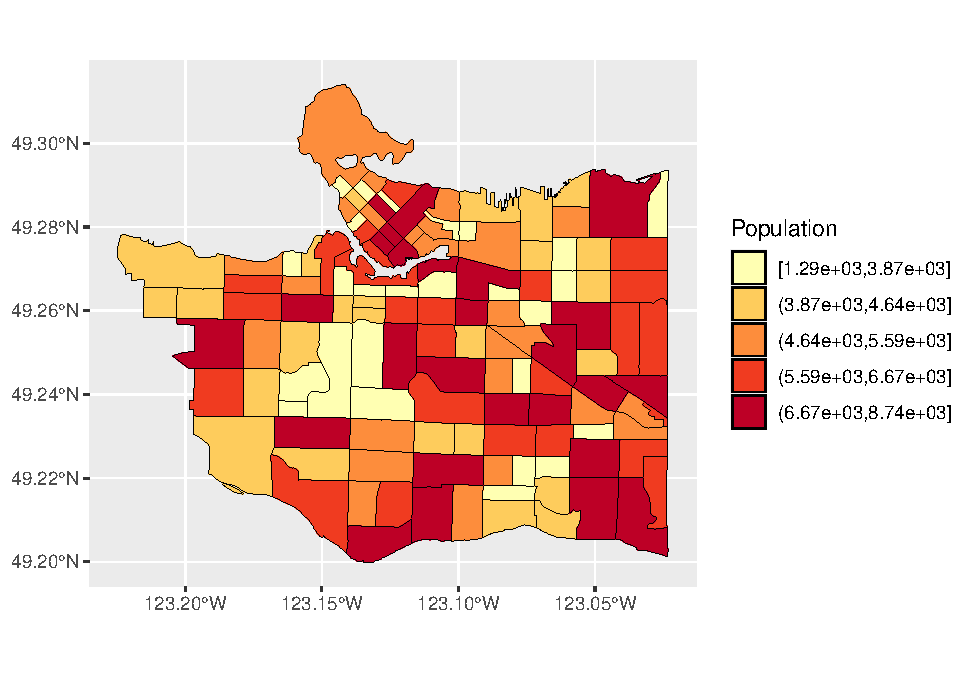
\includegraphics[width=0.8\linewidth]{4GA3Markdown_files/figure-latex/unnamed-chunk-22-1} \end{center}

Population density of each CT

\begin{Shaded}
\begin{Highlighting}[]
\CommentTok{\# creating a choropleth map for the population density}
\FunctionTok{ggplot}\NormalTok{(census\_data) }\SpecialCharTok{+}
  \FunctionTok{geom\_sf}\NormalTok{(}\FunctionTok{aes}\NormalTok{(}\AttributeTok{fill =} \FunctionTok{cut\_number}\NormalTok{(Population\_density, }\DecValTok{5}\NormalTok{)),}
          \AttributeTok{colour =} \StringTok{"black"}\NormalTok{,}
          \AttributeTok{size =} \FloatTok{0.1}\NormalTok{) }\SpecialCharTok{+}
  \FunctionTok{scale\_fill\_brewer}\NormalTok{(}\AttributeTok{palette =} \StringTok{"YlOrRd"}\NormalTok{) }\SpecialCharTok{+}
  \FunctionTok{coord\_sf}\NormalTok{() }\SpecialCharTok{+}
  \FunctionTok{labs}\NormalTok{(}\AttributeTok{fill =} \StringTok{"Population Density"}\NormalTok{)}
\end{Highlighting}
\end{Shaded}

\begin{center}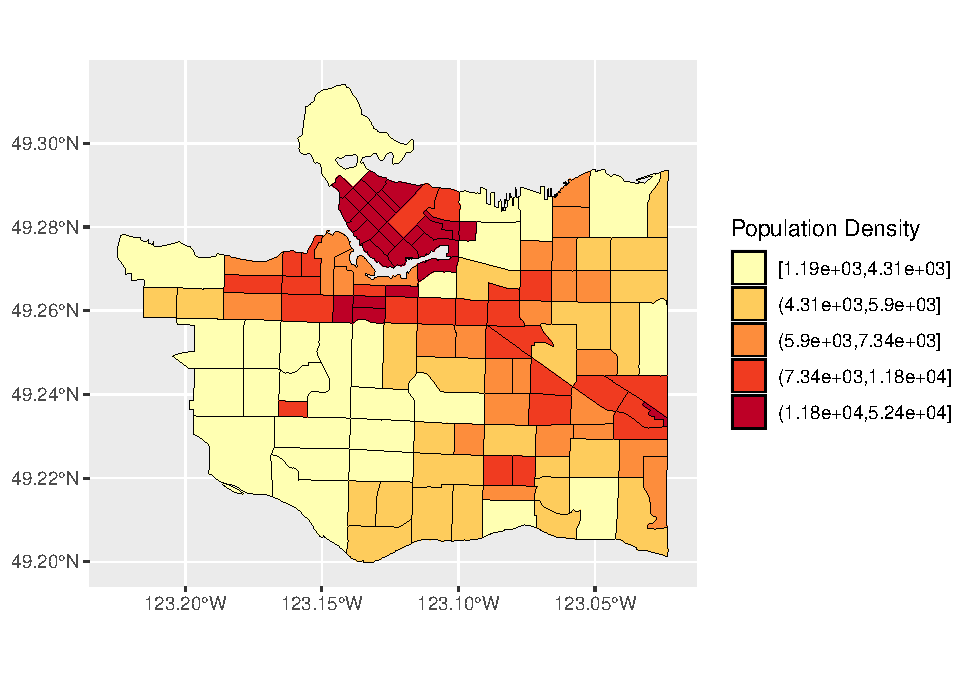
\includegraphics[width=0.8\linewidth]{4GA3Markdown_files/figure-latex/unnamed-chunk-23-1} \end{center}

Proportion of population identifying as visible and non-visible
minorities

\begin{Shaded}
\begin{Highlighting}[]
\CommentTok{\# creating a choropleth map for the proportion of the visisble minority population}
\FunctionTok{ggplot}\NormalTok{(census\_data) }\SpecialCharTok{+}
\FunctionTok{geom\_sf}\NormalTok{(}\FunctionTok{aes}\NormalTok{(}\AttributeTok{fill =} \FunctionTok{cut\_number}\NormalTok{(Proportion\_visible\_minority, }\DecValTok{5}\NormalTok{)),}
        \AttributeTok{color =} \StringTok{"black"}\NormalTok{,}
        \AttributeTok{size =} \FloatTok{0.1}\NormalTok{) }\SpecialCharTok{+}
\FunctionTok{scale\_fill\_brewer}\NormalTok{(}\AttributeTok{palette =} \StringTok{"YlOrRd"}\NormalTok{) }\SpecialCharTok{+}
\FunctionTok{labs}\NormalTok{(}\AttributeTok{fill =} \StringTok{"Prop Visible Minority"}\NormalTok{)}
\end{Highlighting}
\end{Shaded}

\begin{center}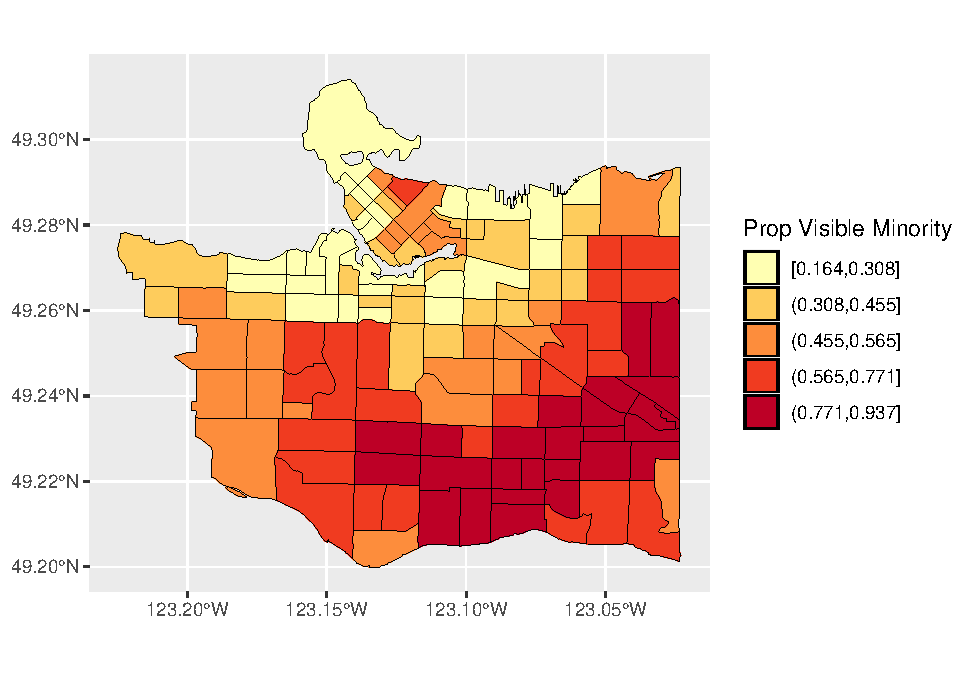
\includegraphics[width=0.8\linewidth]{4GA3Markdown_files/figure-latex/unnamed-chunk-24-1} \end{center}

\begin{Shaded}
\begin{Highlighting}[]
\CommentTok{\# creating a choropleth map for the proportion of the non{-}visible minority population}
\FunctionTok{ggplot}\NormalTok{(census\_data) }\SpecialCharTok{+}
\FunctionTok{geom\_sf}\NormalTok{(}\FunctionTok{aes}\NormalTok{(}\AttributeTok{fill =} \FunctionTok{cut\_number}\NormalTok{(Proportion\_nonvisible\_minority, }\DecValTok{5}\NormalTok{)),}
        \AttributeTok{color =} \StringTok{"black"}\NormalTok{,}
        \AttributeTok{size =} \FloatTok{0.1}\NormalTok{) }\SpecialCharTok{+}
\FunctionTok{scale\_fill\_brewer}\NormalTok{(}\AttributeTok{palette =} \StringTok{"YlOrRd"}\NormalTok{) }\SpecialCharTok{+}
\FunctionTok{labs}\NormalTok{(}\AttributeTok{fill =} \StringTok{"Prop Non{-}Visible Minority"}\NormalTok{)}
\end{Highlighting}
\end{Shaded}

\begin{center}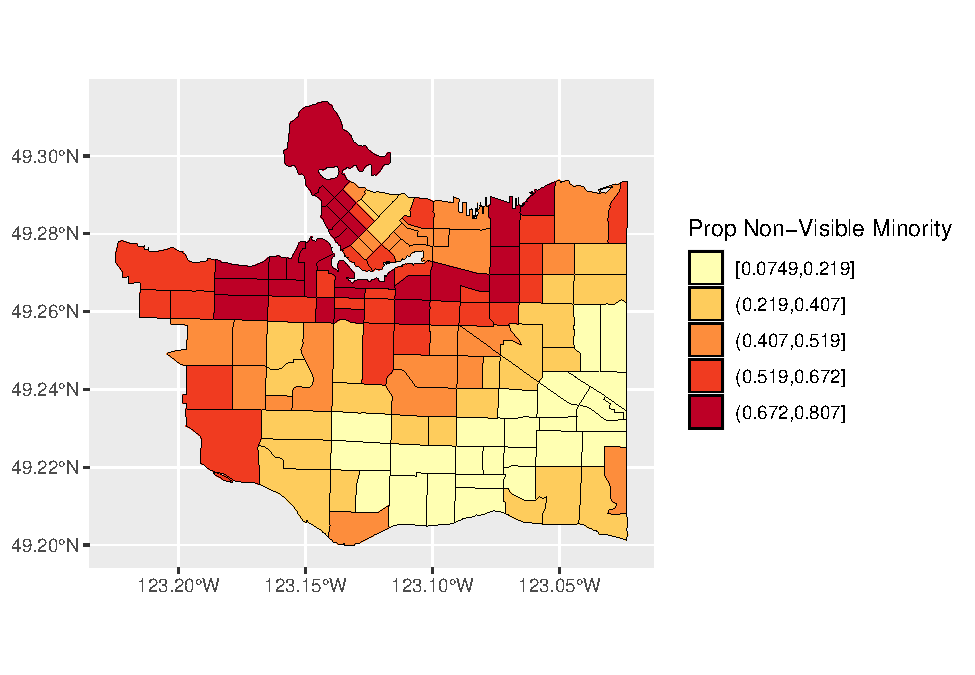
\includegraphics[width=0.8\linewidth]{4GA3Markdown_files/figure-latex/unnamed-chunk-25-1} \end{center}

The proportion of the population considered low income for each CT

\begin{Shaded}
\begin{Highlighting}[]
\CommentTok{\# creating a choropleth map displaying the proportion of low{-}income }
\FunctionTok{ggplot}\NormalTok{(census\_data) }\SpecialCharTok{+}
\FunctionTok{geom\_sf}\NormalTok{(}\FunctionTok{aes}\NormalTok{(}\AttributeTok{fill =} \FunctionTok{cut\_number}\NormalTok{(Proportion\_low\_income, }\DecValTok{5}\NormalTok{)),}
        \AttributeTok{color =} \StringTok{"black"}\NormalTok{,}
        \AttributeTok{size =} \FloatTok{0.1}\NormalTok{) }\SpecialCharTok{+}
\FunctionTok{scale\_fill\_brewer}\NormalTok{(}\AttributeTok{palette =} \StringTok{"YlOrRd"}\NormalTok{) }\SpecialCharTok{+}
\FunctionTok{labs}\NormalTok{(}\AttributeTok{fill =} \StringTok{"Prop Low Income"}\NormalTok{)}
\end{Highlighting}
\end{Shaded}

\begin{center}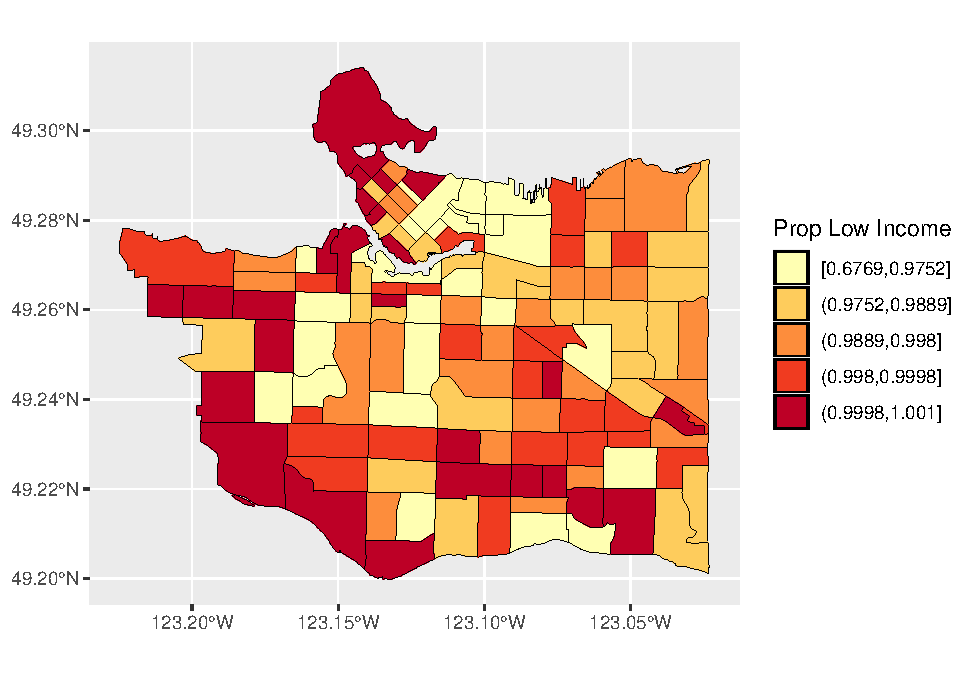
\includegraphics[width=0.8\linewidth]{4GA3Markdown_files/figure-latex/unnamed-chunk-26-1} \end{center}

Finally, a choropleth map was created to display the independent
variable, parks accessible within 30 mintues of a centroid.

\begin{Shaded}
\begin{Highlighting}[]
\CommentTok{\# creating a choropleth map displaying the number of parks accessible to a census tract\textquotesingle{}s centroids within 30 minutes}
\FunctionTok{ggplot}\NormalTok{(census\_data) }\SpecialCharTok{+}
\FunctionTok{geom\_sf}\NormalTok{(}\FunctionTok{aes}\NormalTok{(}\AttributeTok{fill =} \FunctionTok{cut\_number}\NormalTok{(accessibility, }\DecValTok{5}\NormalTok{)),}
        \AttributeTok{color =} \StringTok{"black"}\NormalTok{,}
        \AttributeTok{size =} \FloatTok{0.1}\NormalTok{) }\SpecialCharTok{+}
\FunctionTok{scale\_fill\_brewer}\NormalTok{(}\AttributeTok{palette =} \StringTok{"YlOrRd"}\NormalTok{) }\SpecialCharTok{+}
\FunctionTok{labs}\NormalTok{(}\AttributeTok{fill =} \StringTok{"Number of Neighbourhoods Accessible Within 30 Minutes"}\NormalTok{)}
\end{Highlighting}
\end{Shaded}

\begin{center}\includegraphics[width=0.8\linewidth]{4GA3Markdown_files/figure-latex/unnamed-chunk-27-1} \end{center}

Next, to determine the relationship between the number of accessible
parks and each independent variable, the independent variables were
regressed to number of accessible parks for each CT.

\begin{Shaded}
\begin{Highlighting}[]
\CommentTok{\#creating a regression model of population regressing on number of accessible parks}
\NormalTok{model\_population }\OtherTok{\textless{}{-}} \FunctionTok{lm}\NormalTok{(}\AttributeTok{formula =}\NormalTok{ Population\_2021 }\SpecialCharTok{\textasciitilde{}}\NormalTok{ accessibility, }
             \AttributeTok{data =}\NormalTok{ census\_data)}

\FunctionTok{stargazer}\NormalTok{(model\_population,}
          \AttributeTok{header =} \ConstantTok{FALSE}\NormalTok{,}
          \AttributeTok{title =} \StringTok{"Population of Census Tracts regressed on Number of Parks Accessible"}\NormalTok{)}
\end{Highlighting}
\end{Shaded}

\begin{verbatim}
## 
## \begin{table}[!htbp] \centering 
##   \caption{Population of Census Tracts regressed on Number of Parks Accessible} 
##   \label{} 
## \begin{tabular}{@{\extracolsep{5pt}}lc} 
## \\[-1.8ex]\hline 
## \hline \\[-1.8ex] 
##  & \multicolumn{1}{c}{\textit{Dependent variable:}} \\ 
## \cline{2-2} 
## \\[-1.8ex] & Population\_2021 \\ 
## \hline \\[-1.8ex] 
##  accessibility & 10.518 \\ 
##   & (7.816) \\ 
##   & \\ 
##  Constant & 4,904.639$^{***}$ \\ 
##   & (264.208) \\ 
##   & \\ 
## \hline \\[-1.8ex] 
## Observations & 127 \\ 
## R$^{2}$ & 0.014 \\ 
## Adjusted R$^{2}$ & 0.006 \\ 
## Residual Std. Error & 1,459.451 (df = 125) \\ 
## F Statistic & 1.811 (df = 1; 125) \\ 
## \hline 
## \hline \\[-1.8ex] 
## \textit{Note:}  & \multicolumn{1}{r}{$^{*}$p$<$0.1; $^{**}$p$<$0.05; $^{***}$p$<$0.01} \\ 
## \end{tabular} 
## \end{table}
\end{verbatim}

\begin{Shaded}
\begin{Highlighting}[]
\FunctionTok{summary}\NormalTok{(model\_population)}
\end{Highlighting}
\end{Shaded}

\begin{verbatim}
## 
## Call:
## lm(formula = Population_2021 ~ accessibility, data = census_data)
## 
## Residuals:
##     Min      1Q  Median      3Q     Max 
## -4118.5 -1065.2  -159.5  1192.0  3319.0 
## 
## Coefficients:
##               Estimate Std. Error t value Pr(>|t|)    
## (Intercept)   4904.639    264.208  18.564   <2e-16 ***
## accessibility   10.518      7.816   1.346    0.181    
## ---
## Signif. codes:  0 '***' 0.001 '**' 0.01 '*' 0.05 '.' 0.1 ' ' 1
## 
## Residual standard error: 1459 on 125 degrees of freedom
## Multiple R-squared:  0.01428,    Adjusted R-squared:  0.006395 
## F-statistic: 1.811 on 1 and 125 DF,  p-value: 0.1808
\end{verbatim}

For each regression, a scatter plot was created to provide a visual
representation of the data

\begin{Shaded}
\begin{Highlighting}[]
\FunctionTok{ggplot}\NormalTok{(}\AttributeTok{data =}\NormalTok{ census\_data, }
       \FunctionTok{aes}\NormalTok{(}\AttributeTok{x =}\NormalTok{ accessibility, }
           \AttributeTok{y =}\NormalTok{ Population\_2021))}\SpecialCharTok{+}
  \FunctionTok{geom\_point}\NormalTok{() }\SpecialCharTok{+}
  \FunctionTok{geom\_smooth}\NormalTok{(}\AttributeTok{formula =}\NormalTok{ y }\SpecialCharTok{\textasciitilde{}}\NormalTok{ x,}
              \AttributeTok{method =} \StringTok{"lm"}\NormalTok{) }\SpecialCharTok{+}
  \FunctionTok{ylab}\NormalTok{(}\StringTok{"Population (2021)"}\NormalTok{) }\SpecialCharTok{+}
  \FunctionTok{xlab}\NormalTok{(}\StringTok{"Number of Parks Accessible within 30 Minutes (Through walking or public transit"}\NormalTok{) }
\end{Highlighting}
\end{Shaded}

\begin{center}\includegraphics[width=0.8\linewidth]{4GA3Markdown_files/figure-latex/unnamed-chunk-29-1} \end{center}

Model regressing population density on number of accessible marks

\begin{Shaded}
\begin{Highlighting}[]
\CommentTok{\#creating a regression model of population density regressing on number of accessible parks}
\NormalTok{model\_population\_density }\OtherTok{\textless{}{-}} \FunctionTok{lm}\NormalTok{(}\AttributeTok{formula =}\NormalTok{ Population\_density }\SpecialCharTok{\textasciitilde{}}\NormalTok{ accessibility, }
             \AttributeTok{data =}\NormalTok{ census\_data)}

\FunctionTok{stargazer}\NormalTok{(model\_population\_density,}
          \AttributeTok{header =} \ConstantTok{FALSE}\NormalTok{,}
          \AttributeTok{title =} \StringTok{"Population Density of Census Tracts regressed on Number of Parks Accessible"}\NormalTok{)}
\end{Highlighting}
\end{Shaded}

\begin{verbatim}
## 
## \begin{table}[!htbp] \centering 
##   \caption{Population Density of Census Tracts regressed on Number of Parks Accessible} 
##   \label{} 
## \begin{tabular}{@{\extracolsep{5pt}}lc} 
## \\[-1.8ex]\hline 
## \hline \\[-1.8ex] 
##  & \multicolumn{1}{c}{\textit{Dependent variable:}} \\ 
## \cline{2-2} 
## \\[-1.8ex] & Population\_density \\ 
## \hline \\[-1.8ex] 
##  accessibility & 215.382$^{***}$ \\ 
##   & (39.775) \\ 
##   & \\ 
##  Constant & 2,995.220$^{**}$ \\ 
##   & (1,344.555) \\ 
##   & \\ 
## \hline \\[-1.8ex] 
## Observations & 127 \\ 
## R$^{2}$ & 0.190 \\ 
## Adjusted R$^{2}$ & 0.184 \\ 
## Residual Std. Error & 7,427.142 (df = 125) \\ 
## F Statistic & 29.322$^{***}$ (df = 1; 125) \\ 
## \hline 
## \hline \\[-1.8ex] 
## \textit{Note:}  & \multicolumn{1}{r}{$^{*}$p$<$0.1; $^{**}$p$<$0.05; $^{***}$p$<$0.01} \\ 
## \end{tabular} 
## \end{table}
\end{verbatim}

Scatterplot of population density vs number of accessible parks

\begin{Shaded}
\begin{Highlighting}[]
\FunctionTok{ggplot}\NormalTok{(}\AttributeTok{data =}\NormalTok{ census\_data, }
       \FunctionTok{aes}\NormalTok{(}\AttributeTok{x =}\NormalTok{ accessibility, }
           \AttributeTok{y =}\NormalTok{ Population\_density))}\SpecialCharTok{+}
  \FunctionTok{geom\_point}\NormalTok{() }\SpecialCharTok{+}
  \FunctionTok{geom\_smooth}\NormalTok{(}\AttributeTok{formula =}\NormalTok{ y }\SpecialCharTok{\textasciitilde{}}\NormalTok{ x,}
              \AttributeTok{method =} \StringTok{"lm"}\NormalTok{) }\SpecialCharTok{+}
  \FunctionTok{ylab}\NormalTok{(}\StringTok{"Population Density"}\NormalTok{) }\SpecialCharTok{+}
  \FunctionTok{xlab}\NormalTok{(}\StringTok{"Number of Parks Accessible within 30 Minutes (Through walking or public transit"}\NormalTok{) }
\end{Highlighting}
\end{Shaded}

\begin{center}\includegraphics[width=0.8\linewidth]{4GA3Markdown_files/figure-latex/unnamed-chunk-31-1} \end{center}

Model regressing proportion of visible minorities on number of
accessible parks

\begin{Shaded}
\begin{Highlighting}[]
\CommentTok{\#creating a regression model of population density regressing on number of accessible parks}
\NormalTok{model\_visible\_minority }\OtherTok{\textless{}{-}} \FunctionTok{lm}\NormalTok{(}\AttributeTok{formula =}\NormalTok{ Proportion\_visible\_minority }\SpecialCharTok{\textasciitilde{}}\NormalTok{ accessibility, }
             \AttributeTok{data =}\NormalTok{ census\_data)}

\FunctionTok{stargazer}\NormalTok{(model\_visible\_minority,}
          \AttributeTok{header =} \ConstantTok{FALSE}\NormalTok{,}
          \AttributeTok{title =} \StringTok{"Proportion of Visible Minority Population in Census Tracts regressed on Number of Parks Accessible"}\NormalTok{)}
\end{Highlighting}
\end{Shaded}

\begin{verbatim}
## 
## \begin{table}[!htbp] \centering 
##   \caption{Proportion of Visible Minority Population in Census Tracts regressed on Number of Parks Accessible} 
##   \label{} 
## \begin{tabular}{@{\extracolsep{5pt}}lc} 
## \\[-1.8ex]\hline 
## \hline \\[-1.8ex] 
##  & \multicolumn{1}{c}{\textit{Dependent variable:}} \\ 
## \cline{2-2} 
## \\[-1.8ex] & Proportion\_visible\_minority \\ 
## \hline \\[-1.8ex] 
##  accessibility & $-$0.004$^{***}$ \\ 
##   & (0.001) \\ 
##   & \\ 
##  Constant & 0.654$^{***}$ \\ 
##   & (0.037) \\ 
##   & \\ 
## \hline \\[-1.8ex] 
## Observations & 127 \\ 
## R$^{2}$ & 0.110 \\ 
## Adjusted R$^{2}$ & 0.103 \\ 
## Residual Std. Error & 0.205 (df = 125) \\ 
## F Statistic & 15.511$^{***}$ (df = 1; 125) \\ 
## \hline 
## \hline \\[-1.8ex] 
## \textit{Note:}  & \multicolumn{1}{r}{$^{*}$p$<$0.1; $^{**}$p$<$0.05; $^{***}$p$<$0.01} \\ 
## \end{tabular} 
## \end{table}
\end{verbatim}

Scatterplot of proportion of visible minorities vs number of accessible
parks

\begin{Shaded}
\begin{Highlighting}[]
\FunctionTok{ggplot}\NormalTok{(}\AttributeTok{data =}\NormalTok{ census\_data, }
       \FunctionTok{aes}\NormalTok{(}\AttributeTok{x =}\NormalTok{ accessibility, }
           \AttributeTok{y =}\NormalTok{ Proportion\_visible\_minority))}\SpecialCharTok{+}
  \FunctionTok{geom\_point}\NormalTok{() }\SpecialCharTok{+}
  \FunctionTok{geom\_smooth}\NormalTok{(}\AttributeTok{formula =}\NormalTok{ y }\SpecialCharTok{\textasciitilde{}}\NormalTok{ x,}
              \AttributeTok{method =} \StringTok{"lm"}\NormalTok{) }\SpecialCharTok{+}
  \FunctionTok{ylab}\NormalTok{(}\StringTok{"Proportion of Visible Minority Population"}\NormalTok{) }\SpecialCharTok{+}
  \FunctionTok{xlab}\NormalTok{(}\StringTok{"Number of Parks Accessible within 30 Minutes (Through walking or public transit"}\NormalTok{) }
\end{Highlighting}
\end{Shaded}

\begin{center}\includegraphics[width=0.8\linewidth]{4GA3Markdown_files/figure-latex/unnamed-chunk-33-1} \end{center}

Model regressing proportion of non-visible minorities on number of
accessible parks

\begin{Shaded}
\begin{Highlighting}[]
\CommentTok{\#creating a regression model of population density regressing on number of accessible parks}
\NormalTok{model\_nonvisible\_minority }\OtherTok{\textless{}{-}} \FunctionTok{lm}\NormalTok{(}\AttributeTok{formula =}\NormalTok{ Proportion\_nonvisible\_minority }\SpecialCharTok{\textasciitilde{}}\NormalTok{ accessibility, }
             \AttributeTok{data =}\NormalTok{ census\_data)}

\FunctionTok{stargazer}\NormalTok{(model\_nonvisible\_minority,}
          \AttributeTok{header =} \ConstantTok{FALSE}\NormalTok{,}
          \AttributeTok{title =} \StringTok{"Proportion of Non{-}Visible Minority Population in Census Tracts regressed on Number of Parks Accessible"}\NormalTok{)}
\end{Highlighting}
\end{Shaded}

\begin{verbatim}
## 
## \begin{table}[!htbp] \centering 
##   \caption{Proportion of Non-Visible Minority Population in Census Tracts regressed on Number of Parks Accessible} 
##   \label{} 
## \begin{tabular}{@{\extracolsep{5pt}}lc} 
## \\[-1.8ex]\hline 
## \hline \\[-1.8ex] 
##  & \multicolumn{1}{c}{\textit{Dependent variable:}} \\ 
## \cline{2-2} 
## \\[-1.8ex] & Proportion\_nonvisible\_minority \\ 
## \hline \\[-1.8ex] 
##  accessibility & 0.004$^{***}$ \\ 
##   & (0.001) \\ 
##   & \\ 
##  Constant & 0.336$^{***}$ \\ 
##   & (0.037) \\ 
##   & \\ 
## \hline \\[-1.8ex] 
## Observations & 127 \\ 
## R$^{2}$ & 0.097 \\ 
## Adjusted R$^{2}$ & 0.090 \\ 
## Residual Std. Error & 0.203 (df = 125) \\ 
## F Statistic & 13.473$^{***}$ (df = 1; 125) \\ 
## \hline 
## \hline \\[-1.8ex] 
## \textit{Note:}  & \multicolumn{1}{r}{$^{*}$p$<$0.1; $^{**}$p$<$0.05; $^{***}$p$<$0.01} \\ 
## \end{tabular} 
## \end{table}
\end{verbatim}

Scatterplot of proportion of non-visible minorities vs number of
accessible parks

\begin{Shaded}
\begin{Highlighting}[]
\FunctionTok{ggplot}\NormalTok{(}\AttributeTok{data =}\NormalTok{ census\_data, }
       \FunctionTok{aes}\NormalTok{(}\AttributeTok{x =}\NormalTok{ accessibility, }
           \AttributeTok{y =}\NormalTok{ Proportion\_nonvisible\_minority))}\SpecialCharTok{+}
  \FunctionTok{geom\_point}\NormalTok{() }\SpecialCharTok{+}
  \FunctionTok{geom\_smooth}\NormalTok{(}\AttributeTok{formula =}\NormalTok{ y }\SpecialCharTok{\textasciitilde{}}\NormalTok{ x,}
              \AttributeTok{method =} \StringTok{"lm"}\NormalTok{) }\SpecialCharTok{+}
  \FunctionTok{ylab}\NormalTok{(}\StringTok{"Proportion of Non{-}Visible Minority Population"}\NormalTok{) }\SpecialCharTok{+}
  \FunctionTok{xlab}\NormalTok{(}\StringTok{"Number of Parks Accessible within 30 Minutes (Through walking or public transit"}\NormalTok{) }
\end{Highlighting}
\end{Shaded}

\begin{center}\includegraphics[width=0.8\linewidth]{4GA3Markdown_files/figure-latex/unnamed-chunk-35-1} \end{center}

Model regressing proportion of low income population on number of
accessible parks

\begin{Shaded}
\begin{Highlighting}[]
\CommentTok{\#creating a regression model of population density regressing on number of accessible parks}
\NormalTok{model\_income }\OtherTok{\textless{}{-}} \FunctionTok{lm}\NormalTok{(}\AttributeTok{formula =}\NormalTok{ Proportion\_low\_income }\SpecialCharTok{\textasciitilde{}}\NormalTok{ accessibility, }
             \AttributeTok{data =}\NormalTok{ census\_data)}

\FunctionTok{stargazer}\NormalTok{(model\_income,}
          \AttributeTok{header =} \ConstantTok{FALSE}\NormalTok{,}
          \AttributeTok{title =} \StringTok{"Proportion of Low Income Population in Census Tracts regressed on Number of Parks Accessible"}\NormalTok{)}
\end{Highlighting}
\end{Shaded}

\begin{verbatim}
## 
## \begin{table}[!htbp] \centering 
##   \caption{Proportion of Low Income Population in Census Tracts regressed on Number of Parks Accessible} 
##   \label{} 
## \begin{tabular}{@{\extracolsep{5pt}}lc} 
## \\[-1.8ex]\hline 
## \hline \\[-1.8ex] 
##  & \multicolumn{1}{c}{\textit{Dependent variable:}} \\ 
## \cline{2-2} 
## \\[-1.8ex] & Proportion\_low\_income \\ 
## \hline \\[-1.8ex] 
##  accessibility & $-$0.0004$^{*}$ \\ 
##   & (0.0002) \\ 
##   & \\ 
##  Constant & 0.993$^{***}$ \\ 
##   & (0.008) \\ 
##   & \\ 
## \hline \\[-1.8ex] 
## Observations & 127 \\ 
## R$^{2}$ & 0.028 \\ 
## Adjusted R$^{2}$ & 0.020 \\ 
## Residual Std. Error & 0.041 (df = 125) \\ 
## F Statistic & 3.571$^{*}$ (df = 1; 125) \\ 
## \hline 
## \hline \\[-1.8ex] 
## \textit{Note:}  & \multicolumn{1}{r}{$^{*}$p$<$0.1; $^{**}$p$<$0.05; $^{***}$p$<$0.01} \\ 
## \end{tabular} 
## \end{table}
\end{verbatim}

Scatterplot of proportion of low income population vs number of
accessible parks

\begin{Shaded}
\begin{Highlighting}[]
\FunctionTok{ggplot}\NormalTok{(}\AttributeTok{data =}\NormalTok{ census\_data, }
       \FunctionTok{aes}\NormalTok{(}\AttributeTok{x =}\NormalTok{ accessibility, }
           \AttributeTok{y =}\NormalTok{ Proportion\_low\_income))}\SpecialCharTok{+}
  \FunctionTok{geom\_point}\NormalTok{() }\SpecialCharTok{+}
  \FunctionTok{geom\_smooth}\NormalTok{(}\AttributeTok{formula =}\NormalTok{ y }\SpecialCharTok{\textasciitilde{}}\NormalTok{ x,}
              \AttributeTok{method =} \StringTok{"lm"}\NormalTok{) }\SpecialCharTok{+}
  \FunctionTok{ylab}\NormalTok{(}\StringTok{"Proportion of Low Income Population"}\NormalTok{) }\SpecialCharTok{+}
  \FunctionTok{xlab}\NormalTok{(}\StringTok{"Number of Parks Accessible within 30 Minutes (Through walking or public transit"}\NormalTok{) }
\end{Highlighting}
\end{Shaded}

\begin{center}\includegraphics[width=0.8\linewidth]{4GA3Markdown_files/figure-latex/unnamed-chunk-37-1} \end{center}

\#Analysis

\#Conclusion

\end{document}
